\documentclass[12pt,a4paper]{article}
\usepackage[utf8]{inputenc}
\usepackage[spanish]{babel}
\usepackage{amsmath}
\usepackage{amsfonts}
\usepackage{amssymb}
\usepackage{graphicx}
\usepackage[left=3cm,right=2cm,top=2cm,bottom=2cm]{geometry}
\date{\small{\today}}
\usepackage{fancyhdr}
\usepackage{afterpage}
\usepackage[usenames,dvipsnames,svgnames,table]{xcolor}
\definecolor{gris}{RGB}{220,220,220}



\begin{document}



%caratula
  \begin{center}


    
\includegraphics[scale=0.15]{ib}
    \vspace{1cm}
    \vspace{1cm}
    \\
    \Huge{INSTITUTO BALSEIRO}
    \vspace{2cm}\\
    \huge{\textbf{Ingreso 2019}}\\
    \vspace{1cm}
    \LARGE{Resumen de fórmulas}\\
    \vspace{1cm}
    \large
    \begin{flushleft}

      $-$Autor:\\
      \begin{itemize}

        \item[$+$] Nadia A. Pizarro.

      \end{itemize}

    \end{flushleft}
    \vspace{0,5cm}

    \today
    \thispagestyle{empty}
  \end{center}



\lhead{}
\rhead{Ingreso 2019} % Logo
\chead{Sección: \thesection.\thesubsection}
%\ Pie
\lfoot{Nadia A. Pizarro.}
\cfoot{Instituto balseiro} % quitar número de página del centro
\rfoot{\thepage} % número de página a la derecha
\renewcommand{\headrulewidth}{0.4pt} % grosor de la línea de la cabecera
\renewcommand{\footrulewidth}{0.4pt} % grosor de la línea del pie
\pagestyle{fancy}

%indice

\newpage

\tableofcontents
\newpage

%desarrollo
\begin{quote}
\begin{center}

\abstractname{\textit{ : En el siguiente artículo hare un resumen de las fórmulas y conceptos que repasaré una vez terminado de estudiar todos los temas, no es un resumen de todo lo que sé ni de todo lo que estudié, espero que también le sirva a alguien más.}}

\end{center}
\end{quote}

\section{Análisis Matemático}

\textbf{Derivadas:}
\begin{itemize}
  \item $ \sen(x) \rightarrow \cos(x)$
  \item $ \cos(x) \rightarrow -\sen(x)$
  \item $ \ln(x) \rightarrow \dfrac{1}{x}$
  \item $ \tg(x) \rightarrow \dfrac{1}{\cos^2(x)}$
  \item $ \cotg(x) \rightarrow \dfrac{-1}{\sen^2(x)}$
  \item $ \arcsen(x) \rightarrow \dfrac{1}{\sqrt{1-x^2}}$
  \item $ \arccos(x) \rightarrow \dfrac{-1}{\sqrt{1-x^2}}$
  \item $ \arctg(x) \rightarrow \dfrac{1}{1+x^2}$
\end{itemize}

\textbf{Diferencial:} \\
El valor exacto de un incremento esta dado por $\Delta z = F(x+\Delta x; y +\Delta y )  F(x;y)$ Mientras que podemos obtener un valor aproximado con el diferencial: $dz= \dfrac{\partial F}{\partial x}\cdot dx +\dfrac{\partial F}{\partial y}\cdot dy $. Podemos decir que $\Delta x = dx$ y $\Delta y = dy$ pero $\Delta z \neq dz$, aunque para valores muy pequeños se aproximan.  \\

  \textbf{Dominio de una función:} Debemos restringir el dominio y si se puede graficarlo con las siguientes reglas:
  \begin{itemize}
     \item En los radicales el argumento tiene que ser $ \geq 0$.
     \item El denominador de una fracción debe ser $\neq 0$.
     \item El argumento del logaritmo debe ser $> 0$.

  \end{itemize}

  \textbf{Derivada direccional:}\\
  Se define la derivada direccional de F con respecto al vector $\vec{v}$ como :
  $$\dfrac{\partial F(x;y)}{\partial \vec{v}} = \dfrac{\partial F}{\partial x} \cdot \cos(\alpha)+ \dfrac{\partial F }{\partial y} \cdot \sen(\alpha) $$
  Si el vector $\vec{v}$ esta normalizado se puede escribir como:
  $$\dfrac{\partial F(x;y)}{\partial \vec{v}}=\nabla F \cdot \vec{v}_normalizado$$\\
  De no estar normalizado debemos hacerlo como:
  $$\vec{v}_{normalizado}= \dfrac{\vec{v}}{|\vec{v}|}$$
  \\
  La \textcolor{red}{derivada direccional máxima} es cuando la dirección es la del gradiente en ese punto, mientras que la \textcolor{blue}{derivada direccional mínima} es la misma dirección del gradiente pero de sentido contrario, esto se logra con la multiplicación punto del vector gradiente por el escalar (-1). La \textcolor{green}{derivada direccional nula} será usando un vector tal que sea perpendicular al vector en la derivada direccional máxima.\\

  \textbf{Divergencia:} cambio de densidad en el movimiento de una partícula. Se define con la eq:
 $ \nabla  \cdot \vec{V} = Div \vec{V}$. En la figura \ref{fig:divergencia} se puede observar que quiere decir el escalar que nos dá de resultado.\\

 \begin{figure}[htbp]
   \begin{center}
       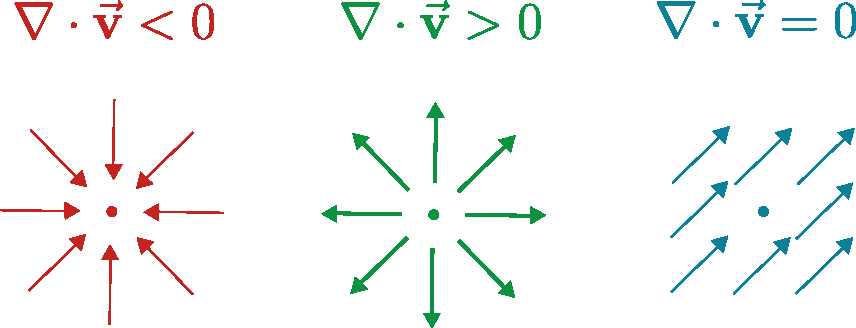
\includegraphics[scale=0.8]{divergencia.pdf}
     \caption{Interpretación de la divergencia}
     \label{fig:divergencia}
   \end{center}
 \end{figure}



 \textbf{Rotacional:} Si una función que toma valores de vectores tridimensionales  $\vec{\textbf{v}}(x,y,z)$ tiene como funciones componentes a $\textcolor{blue}{v_1}(x,y,z)$, $\textcolor{red}{v_2}(x,y,z)$ y $\textcolor{green}{v_3}(x,y,z)$, entonces el rotacional se calcula de la siguiente manera:
$$\nabla \times \vec{\textbf{v}}  = \left( \dfrac{\partial \textcolor{green}{v_3}}{\partial y}- \dfrac{\partial \textcolor{red}{v_2}}{\partial z} \right)\hat{\textbf{i}} + \left( \dfrac{\partial \textcolor{blue}{v_1}}{\partial z}-  \dfrac{\partial \textcolor{green}{v_3}}{\partial x} \right)\hat{\textbf{j}} + \left( \dfrac{\partial \textcolor{red}{v_2}}{\partial x}- \dfrac{\partial \textcolor{blue}{v_1}}{\partial y} \right)\hat{\textbf{k}} $$
\\
Tambien se puede calcular como:
$$\nabla\times \vec{\textbf{v}}=\left|
\begin{matrix} \hat i & \hat j & \hat k  \\ & & \\
\cfrac{\partial}{\partial x} & \cfrac{\partial}{\partial y} & \cfrac{\partial}{\partial z}
\\ & & \\ \textcolor{blue}{v_1} & \textcolor{red}{v_2} & \textcolor{green}{v_3}  \end{matrix}\right|$$
\\


\textbf{Teorema fundamental del cálculo:} Dada unafunción $f$ integrable sobre el intervalo $ [a,b]$, definimos $F$ sobre $[a,b]$ por $F(x) = {\int_{a}^x f(t)dt}$. Si $f$ es continua en $c \notin (a,b)$, entonces $F$ es derivable en $c$ y $F'(c) = f(c)$.\\

\textbf{Plano tangente:} La ecuación del plano tangente de la gráfica de una función de dos variables f(x,y) en un punto particular $(x_0, y_0)$ se ve así:
$$T(x, y) = f(x_0, y_0) + {f_{\textcolor{blue}{x}}(x_0, y_0)}(\textcolor{blue}{x}-x_0) + {f_{\textcolor{red}{y}}(x_0, y_0)}(\textcolor{red}{y}-y_0) $$



\end{document}
